\documentclass[11pt]{article}
\usepackage[utf8]{inputenc}
\usepackage{mathptmx}

% Overall doc formatting 
\addtolength{\oddsidemargin}{-.875in}
\addtolength{\evensidemargin}{-.875in}
\addtolength{\textwidth}{1.75in}
\addtolength{\topmargin}{-.875in}
\addtolength{\textheight}{1.75in}

% To remove section numbering but keep the contents table
\makeatletter
\renewcommand{\@seccntformat}[1]{}
\makeatother

% Para formatting including indentation
\setlength{\parindent}{4em}
\setlength{\parskip}{1em}
\renewcommand{\baselinestretch}{1.0}

% To enable indentation on first para
\usepackage{indentfirst}

% For pictures
\usepackage{graphicx}


\title{Fitness Logger Mid-term Report}
\author{Dumitru Vulpe}
\date{January 2021}

\begin{document}

\maketitle
\tableofcontents
\newpage

\section{Project Summary}

Here I will be outlining what the purpose of my project is, including some technical detail about how the backend will be implemented. The purpose of this project is more of a proof of concept and a learning experience rather then a practical way to implement this project in this way. \par

The base concept is to just be a fitness logging application which you would then be able to use to generate graphs and trends to see the progress. This project is meant to be made in a manner which allows a great deal of flexibility when in comes to the types of logs entered by the user. The frontend will just be mostly an Android app which will be mostly made up of forms and will also have a trends section. If time allows it, I will also be implementing a web frontend to be used as an admin console. In this project, the backend is the most complex part and will take the most amount of effort and research. Simply because the backend will be implemented with micro services. \par

\section{Background Research}

The background market research for this project just consisted of searching and trying out different workout apps. However most of them tend to have either bug, or force you to follow a specific program, or do not have the ability to specific (custom) elements of an exercise. The problem is that there a lot of different aspect which could be logged, this is the reason why most athletes, or average gym goers which log workouts use notebooks in order to customise the log level to their needs.  \par

The specific gap in the market which this project is attempting to fill is to make a simple, yet customisable fitness/workout logger which will let you create an entry, say ``bench press'' or ``caffeine'' (consumed before a workout), customise the values entered for each entry (for example for ``bench press'' have sets, which would have number of reps and a weight value in kg and for ``caffeine'' enter in the amount in mg), then repeatedly be able to enter values and track it overtime. \par

\section{Main Features}

Be able to create different ``tracking points'' or as referred to them above, entries, with different properties. Be able to enter individual entries for those ``tracking points'' in organised groups. After witch, the app would be able to generate trends to visualise the progress. \par

\section{Current Progress}

Since I did not have any prior micro services experience I first had to start by researching the topic. Then I quickly started putting together ideas about how I would like to organise my project, technology I would be using and more. After the research part I started creating the main repo I would be using and setup subsequent sub-module repositories for the different sub components. \par

In terms of the actual coding, so far the shared library which will mainly be used has been setup and appropriately linked so that it can be used by the rest of the micro services. Next, the main template for services started coming together with all of the libraries that I would need. \par

The main language for this project is Nodejs with typescript. However, one common assumption which we have about micro services development is that we can easily interchange libraries, languages and frameworks since we will be writing multiple programs, so as a part of my proof of concept, I wanted to test that and written my first micro service in GoLang. \par

The first micro service is for authentication. It's main functionality is to just register users and create JWT tokens for them (at the login stage). This is the base functionality of it, and at the moment I do not plan to be adding any more features to it, I already had some in mind which would be nice to have. One of them is adding state like functionality side by side with the JWT token system. This would be nice in terms use user account management and to have the ability to logout. \par


\section{Personal Reflection}

\subsection{Main Challenges}
The main challenges which I had until now were to do mostly with all of the research into the topic of micro services and the amount of options there are when designing a project using this system. This challenge was amplified due to the fact that there does not exist a standard way of designing micro services and I had no previous experience with them. I also had to learn more specific stuff which was a bit tricky to get a hold of. For example, learning how to make a shared library in Nodejs with typescript.\par

\subsection{My Thoughts}
This project is still far from being finished. The actual development for the functionality needed being started only in mid January. The parts to be completed come as follows: database design, database implementation, the actual micro services, the frontend app, deployment in Kubernetes, and micro service logging. In terms of the timeline for this project, the plan is to finish implementing all the core parts of this project before the end of March, this is so that there is enough time for deployment, troubleshooting and report writing in April. This will definitely be a bit of a crunch, however, this should not be a problem.\par

\newpage
\section{Conclusion}

\begin{center}
    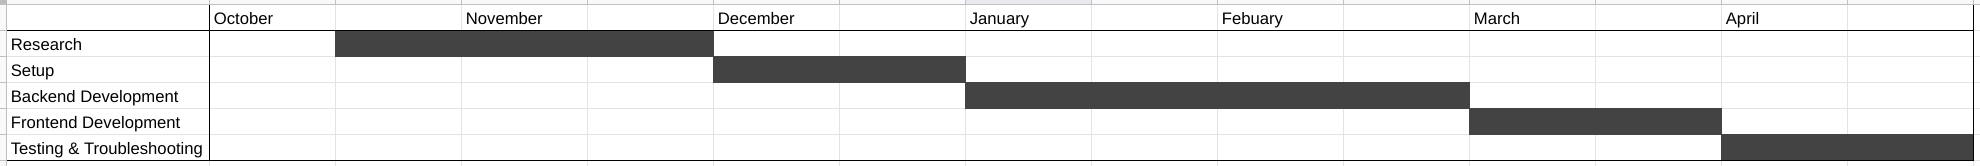
\includegraphics[scale=0.4]{GanttChart}
    Gantt Chart\par
\end{center}

The main milestones I have are the ones in the Gantt Chart: research, setup, backend development, frontend development and testing \& troubleshooting. Right now I am in the backend development phase. And the reason why it is the longest is simply because along side writing all the micro services I will also have to setup a Kubernetes deployments. When it comes to the frontend development, there is only one main app which I will be developing to consume the API If given enough time I will also be developing an admin console for metrics and any administration purposes. The testing and troubleshooting phase is there for fixing last minute problems, testing the application (end to end and possible user testing) and for writing the final report. \par

I am confident in being able to finish the application, however, my main risk is simply time. I might not be able to fully finish the frontend application. So far, I seem to be on track.\par

\end{document}

